\documentclass{article}
\usepackage{graphicx} % Required for inserting images
\usepackage{indentfirst}
\usepackage{hyperref}
% \usepackage{lipsum}
\usepackage{float}
\usepackage{amsthm}
\usepackage{amsmath,amssymb}

\theoremstyle{definition}
\newtheorem{definition}{Definition}[section]
\newtheorem{lemma}{Lemma}[section]

% \title{To what extent can Fourier Analysis be used to solve Ordinary Differential Equations and Partial Differential Equations?}
% \author{Saptak Das}
% \date{June 2023}

\begin{document}
%TC:ignore
\begin{titlepage}
    \begin{center}
        \null
        \vfill
            
        \Large
        \textbf{To what extent, can Fourier Analysis be used to solve Ordinary Differential Equations and Partial Differential Equations?}
            
        \vspace{0.5cm}
        
        \large
        % \textbf{Saptak Das} 
        
        June 2023

        \vspace{2cm}

        Subject: Mathematics

        Word Count: xxxx
        
        \vfill
    \end{center}
\end{titlepage}
%TC:endignore

\tableofcontents
\newpage

\section{Introduction}
\label{section:introduction}
This year I utilized differential equations to come up with the following accurate and applicable epidemic model for policymakers that accounts for disease incubation, quarantine, immunity wear-off, and mortality rates.

\[ \frac{dS}{dt} = -\frac{\beta S I}{N} + \mu R \]
\[ \frac{dE}{dt} = \frac{\beta S I}{N} - \phi E \]
\[ \frac{dI}{dt} = \phi E - \zeta I - \gamma I - \alpha I \]
\[ \frac{dQ}{dt} = \zeta I - \kappa Q - \epsilon Q \]
\[ \frac{dR}{dt} = \gamma I + \kappa Q - \mu R \]
\[ \frac{dD}{dt} = \alpha I + \epsilon Q \]

\noindent
where:
\begin{itemize}
    \item $N$ is the total population.
    \item $\beta$ is the contact rate (1/days).
    \item $\phi$ is the incubation rate (1/days).
    \item $\zeta$ is the quarantine rate (1/days).
    \item $\gamma$ is the recovery rate (non-quarantine) (1/days).
    \item $\kappa$ is the recovery rate (quarantine) (1/days).
    \item $\mu$ is the immunity wearoff rate (1/days).
    \item $\alpha$ is the case fatality rate (non-quarantine) (1/days).
    \item $\epsilon$ is the case fatality rate (quarantine) (1/days).
\end{itemize}

% \lipsum[3]

\section{Background}
\label{section:background}
\subsection{Differential Equations}
\subsubsection{Why are Differential Equations important?}
Calculus is the mathematics of change. Hence, differential equations, which relate the derivatives or integrals of a function to the function itself, can very elegantly summarize the behavior of otherwise complex, dynamic systems. As a result, differential equations are extremely powerful in their ability to model various systems in applied mathematics, physics, and engineering.

For example, the Lotka-Volterra equations describe the dynamics of populations of predators and prey. These equations are described below \citep{wangersky1978lotka}.

\begin{align}
    \frac{dx}{dt} &= \alpha x - \beta x y \label{eq:lotka_volterra_1} \\
    \frac{dy}{dt} &= \delta x y - \gamma y \label{eq:lotka_volterra_2}
\end{align}

\noindent
where:
\begin{itemize}
    \item $x$ is the population density of the prey.
    \item $y$ is the population density of the predator.
    \item $\alpha$ is the exponential growth rate of the prey.
    \item $\gamma$ is the exponential decay rate of the predators.
    \item $\beta$ is the effect of the predators on the prey growth rate.
    \item $\delta$ is the effect of the presence of prey on the predator growth rate.
\end{itemize}

\noindent
\cref{eq:lotka_volterra_1,eq:lotka_volterra_2} are a set of first-order, nonlinear ODEs. This is further explained in \cref{subsubsection:properties_differential} \nameref{subsubsection:properties_differential}.

\subsubsection{Properties of Differential Equations}
\label{subsubsection:properties_differential}
\begin{definition}
    The order of a system of differential equations is defined as the highest-order derivative the system contains. Since the highest order derivative in the Lotka-Volterra \cref{eq:lotka_volterra_1,eq:lotka_volterra_2} is $\frac{d}{dt}$, the equations are first-order.
\end{definition}

\begin{definition}
    If \(x_1(t)\) and \(x_2(t)\) are both solutions to a linear system of differential equations, then any linear superposition is also a solution to the system, namely anything in the form:
    \begin{equation}
        x(t) = c_1 x_1(t) + c_2 x_2(t) 
    \end{equation}
    More formally, a system of differential equations is said to be linear if and only if the equations follows the form:
    \begin{equation}
        a_0 y + a_1 y' + a_2 y'' \dots + a_n y^{(n)} = b(x)
    \end{equation}
    \noindent
    where $a_0, a_1, a_2, ..., a_n$ are any differentiable functions (do not need to be linear).
\end{definition}

\subsubsection{Solution to Differential Equations}
Note that the solution to a differential equation is not one function, but rather a set of functions that all satisfy the differential equation. Some initial conditions must be given to reduce the solution to a single function. For example, for the Lotka-Volterra equations, the phase space shown in \cref{fig:lotka_volterra_phase} plots the various function solutions given various different initial conditions. The smaller loops represent a small predator-prey environment, while the larger loops represent a large predator-prey environment. The solution for a specific initial condition over time is plotted in \cref{fig:lotka_volterra_init}.

\begin{figure}[H]
    \centering
    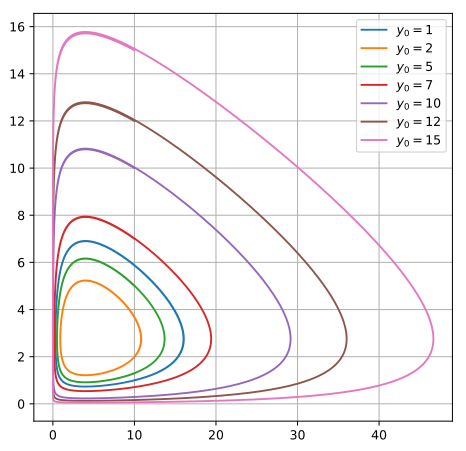
\includegraphics[width=75mm,height=\textheight,keepaspectratio]{images/Predator_prey_dynamics.png}
    \caption{Solution to the Lotka-Volterra Equations given different predator initial conditions.}
    \label{fig:lotka_volterra_phase}
\end{figure}

\begin{figure}[H]
    \centering
    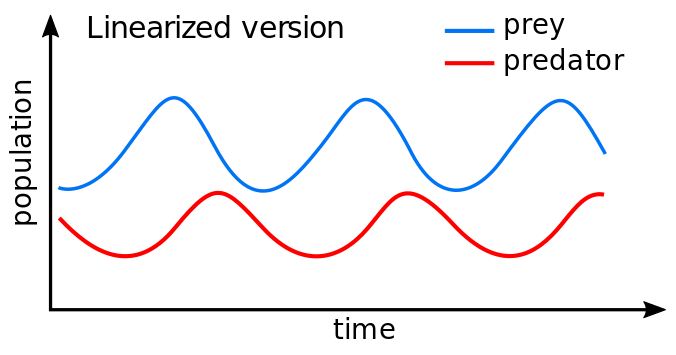
\includegraphics[width=75mm,height=\textheight,keepaspectratio]{images/Lotka_Volterra_dynamics.png}
    \caption{Solution to the Lotka-Volterra Equations given some initial conditions. The predator population function lags behind the prey population as an increase in the prey causes a proportional increase in the predator. Specifically, the predator function is shifted $\frac{\pi}{2}$ radians right of the prey function.}
    \label{fig:lotka_volterra_init}
\end{figure}

\subsubsection{ODE vs PDE}
The Lotka-Volterra Equations are a system of Ordinary Differential Equations (ODEs). This means that the prey population \(x\) and the predator population \(y\) are solely functions of time \(t\).

However, not all functions will be a function of solely one variable such as time or space. For example, \(f(x, t)\) could represent a function dependent on both a position \(x\) and a time \(t\). In this case, Partial Differential Equations (PDEs) could be written using partial derivatives to express the gradient for the multivariate function with respect to a specific variable. \cref{eq:trivial_pde} below is a trivial PDE.

\begin{align}
    \frac{\partial f}{\partial x} = \frac{\partial f}{\partial t} = 0 \label{eq:trivial_pde}
\end{align}


\subsection{Fourier Analysis}
\subsubsection{What is Fourier Analysis?}
Fourier Analysis is a field of mathematics that studies how complex function waveforms can be decomposed into a series of sinusoidal functions, whose frequencies form a harmonic series. In other words, the Fourier Series and Fourier Transform, the cornerstones of Fourier Analysis, turn a signal in time-space respectively into a signal in frequency space and a signal in real space into a signal in Fourier space \citep{stein2011fourier}.

\subsubsection{Difference between Fourier Series and Fourier Transform}
 Fourier series focuses on periodic functions and aims to represent them as a sum of sinusoidal functions (sine and cosine). It decomposes a periodic signal into a combination of harmonically related sine and cosine waves, revealing the frequency components present in the signal. On the other hand, Fourier transforms extend this idea to non-periodic signals or functions, allowing for the analysis of signals that do not repeat in a periodic manner. Fourier transforms provide a continuous spectrum representation of a signal in terms of frequency, capturing both the amplitude and phase information across all frequencies \citep{Tutorialspoint_2022}.

\subsubsection{Fourier Series}
\noindent
Let \(f(x)\) be defined as the following periodic, yet discontinuous square waveform signal (Heaviside Step Function) \citep{Mathworld_2023b}:

\begin{equation} \label{eq:heaviside_step}
f(x)=
    \begin{cases}
        1 & \text{if } nT < x < \frac{T(2n+1)}{2} , n \in \mathbb{Z}\\
        0 & \text{if } x = \frac{nT}{2} , n \in \mathbb{Z}\\
        -1 & \text{if } \frac{T(2n+1)}{2} < x < T(n+1) , n \in \mathbb{Z}
    \end{cases}
\end{equation}

\noindent
In order to obtain the Fourier Series for \(f(x)\), the Fourier Transform of \(f(x)\) must be taken \citep{Tutorialspoint_2022}.

\begin{figure}[H]
    \centering
    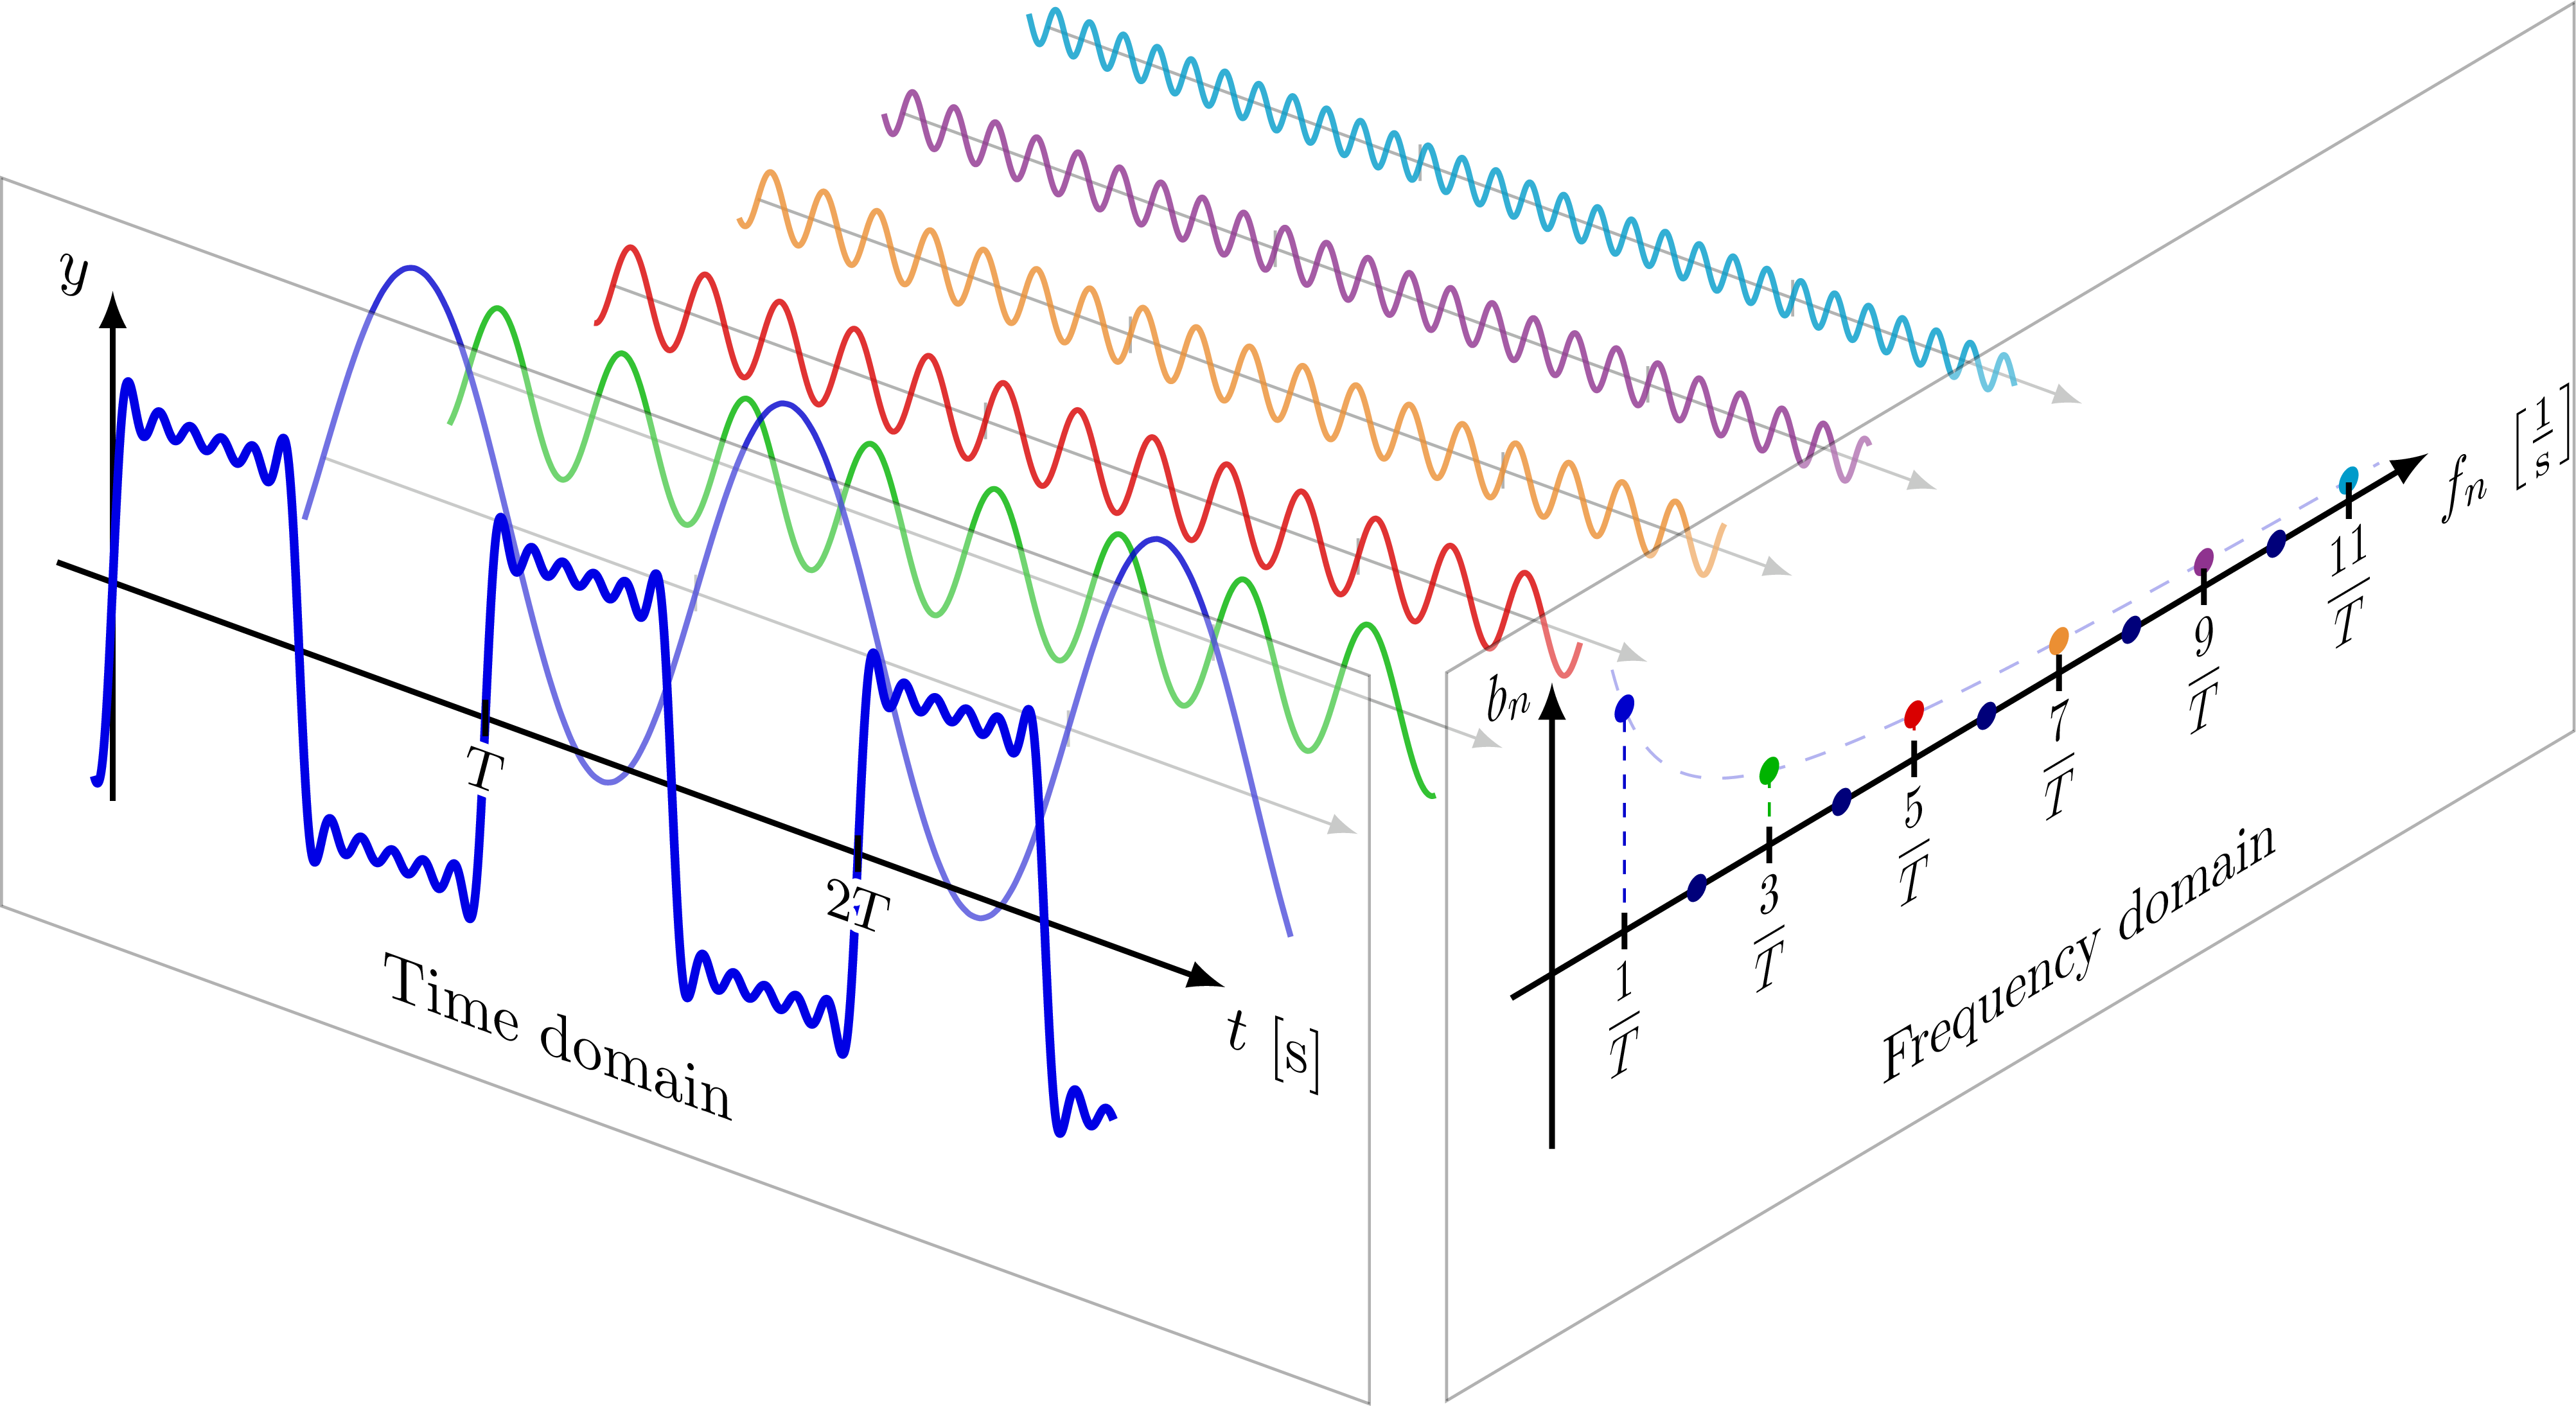
\includegraphics[width=100mm,height=\textheight,keepaspectratio]{images/step_function_fourier_series.png}
    \caption{On the axis to the right, the Fourier Transform of \(f(x)\) can be seen. If an infinite summation of all the frequencies with their corresponding amplitudes was performed as defined by the Fourier Transform, the solution would be exactly equal to \(f(x)\).}
    \label{fig:decomposed_step_function}
\end{figure}

\noindent
Therefore, f(x) (\cref{eq:heaviside_step}) can be defined by the infinite summation of sine functions through its Fourier Series as follows: 
\begin{equation}
    f(x)=\frac{4}{\pi}\sum_{n=1,3,5,...}^{\infty} \frac{1}{n} \sin \left( \frac{2 \pi n x}{T}
 \right)
\end{equation}

\subsubsection{Fourier and Inverse Fourier Transforms}
\begin{definition}
    For a continuous function $f(x)$, the Continuous Fourier Transform $\mathcal{F}\{ f(x) \}$ (CFT) is defined as below \citep{grafakos2008classical}. The transform returns the frequency space function $F(\omega)$.
    \begin{equation} \label{eq:fourier_transform}
        F(\omega) = \mathcal{F}\{ f(x) \} = \int_{-\infty}^{\infty} f(x)  \, e^{-i \omega x} \,dx
    \end{equation}
\end{definition}

%%%%%%%%%%%%%%%%%%%%%%%%%%%%%%%%%%%%%%%%%%%%%%%%%%%%%%%%%%%%%%%%%%%%%%%%%%%%%%%%

\begin{definition}
    In order to reverse the Fourier Transform, the Inverse Continuous Fourier Transform $\mathcal{F}^{-1}\{ F(\omega) \}$ (ICFT) can be applied as defined below \citep{grafakos2008classical}.
    \begin{equation} \label{eq:inverse_fourier_transform}
        f(x) = \mathcal{F}^{-1}\{ F(\omega) \} = \frac{1}{2\pi} \int_{-\infty}^{\infty} F(\omega) \, e^{i \omega x} \,d \omega
    \end{equation}
\end{definition}

\subsubsection{Properties of the Fourier Transform}
The Fourier Transform, which is a coordinate transform, is important and useful because many mathematical operations in Fourier space are simplified compared to the original space. Below are some of the important properties of the Fourier Transform that will be useful in solving differential equations using Fourier Analysis \citep{bahouri2011fourier, 3Blue1Brown_fourier_2018}.
\begin{lemma}
    \label{fourier_scaling}
    If a function \(f(x)\) is scaled by a constant $a$, the Fourier Transform will also be scaled by $a$.
    \begin{equation}
        \mathcal{F}\{ a f(x) \} = a \mathcal{F}\{ f(x) \}
    \end{equation}
\end{lemma}

\begin{proof}
    \begin{align*}
        \mathcal{F}\{ a f(x) \} &= \int_{-\infty}^{\infty} a f(x) \, e^{-i \omega x} \,dx \\
        &= a \int_{-\infty}^{\infty} f(x) \, e^{-i \omega x} \,dx \\
        &= a \mathcal{F}\{ f(x) \}
    \end{align*}
\end{proof}

%%%%%%%%%%%%%%%%%%%%%%%%%%%%%%%%%%%%%%%%%%%%%%%%%%%%%%%%%%%%%%%%%%%%%%%%%%%%%%%%

\begin{theorem}
    \label{fourier_linearity}
    The Fourier Transform is a linear transformation. This means that the transform of a linear combination of functions is equal to the linear combination of the transforms of the individual functions \citep{bahouri2011fourier, 3Blue1Brown_fourier_2018}.
    \begin{equation}
        \mathcal{F}\{ a f(x) + b g(x) \} = a \mathcal{F}\{ f(x) \} + b \mathcal{F}\{ g(x) \}
    \end{equation}
\end{theorem}
\begin{proof}
    \[ \mathcal{F}\{ a f(x) + b g(x) \} = \int_{-\infty}^{\infty} (a f(x) + b g(x)) \, e^{-i \omega x} \,dx \]
    \[ = \int_{-\infty}^{\infty} a f(x) \, e^{-i \omega x} \,dx + \int_{-\infty}^{\infty} b g(x) \, e^{-i \omega x} \,dx \]
    Using \cref{fourier_scaling},
    \begin{align*}
        &= a \int_{-\infty}^{\infty} f(x) \, e^{-i \omega x} \,dx + b \int_{-\infty}^{\infty} g(x) \, e^{-i \omega x} \,dx \\
        &= a \mathcal{F}\{ f(x) \} + b \mathcal{F}\{ g(x) \}
    \end{align*}
\end{proof}

%%%%%%%%%%%%%%%%%%%%%%%%%%%%%%%%%%%%%%%%%%%%%%%%%%%%%%%%%%%%%%%%%%%%%%%%%%%%%%%%

\begin{theorem}
    \label{fourier_shift}
    The Fourier Transform can be shifted easily along the axis of the transform. When a function \(f(x)\) along the x-axis by \(x_0\) units, the transform of the shifted function is equal to the transform of the original function multiplied by $e^{-i \omega x_0}$ \citep{bahouri2011fourier, 3Blue1Brown_fourier_2018}.
    \begin{equation}
        \mathcal{F}\{ f(x - x_0) \} = e^{-i \omega x_0} F(\omega)
    \end{equation}
\end{theorem}

\begin{proof}
    \[ \mathcal{F}\{ f(x - x_0) \} = \int_{-\infty}^{\infty} f(x - x_0) \, e^{-i \omega x} \,dx \]
    Let \(u = x - x_0\). Thus, \(x = u + x_0\) and \(dx = du\).
    \begin{align*}
        &= \int_{-\infty}^{\infty} f(u) \, e^{-i \omega (u + x_0)} \,du \\
        &= e^{-i \omega x_0} \int_{-\infty}^{\infty} f(u) \, e^{-i \omega u} \,du \\
        &= e^{-i \omega x_0} F(\omega)
    \end{align*}
\end{proof}

%%%%%%%%%%%%%%%%%%%%%%%%%%%%%%%%%%%%%%%%%%%%%%%%%%%%%%%%%%%%%%%%%%%%%%%%%%%%%%%%
\begin{theorem}
    \label{fourier_derivative}
    The Fourier Transform of a function's derivative is equal to the transform of the original function multiplied by $i \omega$ \citep{bahouri2011fourier, 3Blue1Brown_fourier_2018}.
    \begin{equation}
        \mathcal{F}\{ \frac{d f(x)}{dx} \} = i \omega \mathcal{F}\{ f(x) \}
    \end{equation}
\end{theorem}

\begin{proof}
    \[ \mathcal{F}\{ \frac{d f(x)}{dx} \} = \int_{-\infty}^{\infty} \frac{d f(x)}{dx}  \, e^{-i \omega x} \,dx \]
    Using integration by parts, let \(u = f(x)\) and \(dv = e^{-i \omega x} dx\).
    \[ = \left[ f(x) e^{-i \omega x} \right]_{-\infty}^{\infty} - \int_{-\infty}^{\infty} f(x) \left( \frac{d}{dx} e^{-i \omega x} \right) \,dx \]
    Since \(f(x)\) must be continuous and integrable to be differentiable and take the Fourier Transform on \(\mathbb{R}\), \(\lim_{x \to -\infty} f(x)=\lim_{x \to \infty} f(x)=0\) must be true. Thus, the first term is equal to zero. 
    \begin{align*}
        &= - \int_{-\infty}^{\infty} f(x) \left( -i \omega e^{-i \omega x} \right) \,dx \\
        &= i \omega \int_{-\infty}^{\infty} f(x) e^{-i \omega x} \,dx \\
        &= i \omega \mathcal{F}\{ f(x) \}
    \end{align*}
\end{proof}

%%%%%%%%%%%%%%%%%%%%%%%%%%%%%%%%%%%%%%%%%%%%%%%%%%%%%%%%%%%%%%%%%%%%%%%%%%%%%%%%
\begin{theorem}
    \label{fourier_multiplication}
    The Fourier Transform of the product of two functions is equal to the convolution of the transforms of the individual functions over \(2 \pi\) \citep{bahouri2011fourier, 3Blue1Brown_fourier_2018}.
    \begin{equation}
        \mathcal{F}\{ f(x) g(x) \} = \frac{1}{2 \pi}( F(\omega) * G(\omega) )
    \end{equation}
\end{theorem}

\begin{proof}
    \[ \mathcal{F}\{ f(x) g(x) \} = \int_{-\infty}^{\infty} f(x) g(x) \, e^{-i \omega x} \,dx \]
    From the definition of the inverse Fourier Transform in \cref{eq:inverse_fourier_transform},
    \[ = \frac{1}{2 \pi} \int_{-\infty}^{\infty} \left( \int_{-\infty}^{\infty} F(\kappa) e^{i \kappa x} \,d\kappa \right) g(x) \, e^{-i \omega x} \,dx \]
    Using Fubini's Theorem, we can switch the order of integration.
    \begin{align*}
        &= \frac{1}{2 \pi} \int_{-\infty}^{\infty} F(\kappa) \left( \int_{-\infty}^{\infty} g(x) e^{-i \omega x} e^{i \kappa x} \,dx \right) \,d\kappa \\
        &= \frac{1}{2 \pi} \int_{-\infty}^{\infty} F(\kappa) \left( \int_{-\infty}^{\infty} g(x) e^{-i (\omega - \kappa) x} \,dx \right) \,d\kappa \\
        &= \frac{1}{2 \pi} \int_{-\infty}^{\infty} F(\kappa) G(\omega - \kappa) \,d\kappa
    \end{align*}
    Given the definition of convolution of two functions \(f(x)\) and \(g(x)\) as:
    \[ f(x) * g(x) = \int_{-\infty}^{\infty} f(\kappa) g(x-\kappa) \,d\kappa \]
    The Fourier Transform of the product of two functions is equal to the convolution of the transforms of the individual functions over \(2 \pi\).
    \[ \mathcal{F}\{ f(x) g(x) \} = \frac{1}{2 \pi}( F(\omega) * G(\omega) ) \]
\end{proof}
\section{Exploration of Applications}
\subsection{The Heat Equation}
Fourier Analysis was first discovered when Joseph Fourier first developed the Heat Equation. The Heat Equation models the flow of heat along a certain heat profile over time. In this example, a 1D solution will be derived and solved.

\subsubsection{Brief Derivation}

\subsubsection{Application of the Fourier Transform}

\subsubsection{Final Solution}


\end{document}
